\section{Experimental evaluation}\label{sec:experimental-evaluation}

\subsection{Experiment setup}

\subsubsection{Datasets}

The proposed methods were experimentally verified on several datasets. The datasets Cora and CiteSeer \cite{yang_revisiting_2016} were used with the \enquote{full} train-test split as in \cite{chen_fastgcn_2018}, as well as the Enzymes dataset \cite{morris_tudataset_2020}, where only the 100 largest datsets were selected and used for training, validation and testing with a random 60:20:20 split. Two larger datasets were also used, the PubMed dataset \cite{yang_revisiting_2016} containing 19 717 nodes and 88 648 edges, and the DBLP dataset \cite{bojchevski_deep_2018} containing 17 716 nodes and 105 734 edges.

\subsubsection{Methodology of experiments}

The hyper-parameters for both the node2vec model used for the embedding training and the multi-layer perceptron used for downstream classification were initially set to values used in prior art (see \cite{hu_open_2021, fey_fast_2019}) and then manually fine-tuned for each dataset.

For the Cora dataset, the node2vec model generated an embedding into \( \mathfield{R}^{128} \) from \( 4 \) random walks of length \( 20 \) for each node with a context window of size \( 5 \). The optimizer ADAM \cite{kingma_adam:_2017} was used with a learning rate of \( 0.01 \) and batches of \( 128 \) samples. The model was trained for \( 5 \) epochs and in each step of the adaptive prolongation, \( 100 \) nodes were prolonged, until reaching the original graph. The MLP classifier using the embeddings featured \( 3 \) linear layers of \( 128 \) neurons with batch normalization after each layer. Each layer was normalized using dropout \cite{srivastava_dropout_2014} with the rate of \( 0.5 \). Finally, a linear layer was used for the class prediction. ADAM with a learning rate of \( 0.01 \) was used for \( 30 \) epochs of training with the cross-entropy loss function. Dataset features weren't used for the classifier training as the aim of this work is to compare the embeddings. The experiment was run \( 10 \) times end-to-end and results averaged. For other datasets, the overall design of the experiment was identical, with the only difference being in the values of some hyper-parameters. Additionally, for the Enzymes datasets, the results were not averaged across multiple runs, but across testing graphs instead. The hyper-parameter values for all datasets are listed in Table \ref{tab:hyperparameter-values}. The experiments were implemented using PyTorch \cite{paszke_pytorch_2019} and PyTorch Geometric \cite{fey_fast_2019}.

\begin{table}
  \caption{Hyper-parameter values used for different datasets}
  \label{tab:hyperparameter-values}
  \begin{tabular}{lrrrrr}
    \toprule
    \textbf{Hyper-parameter} & \textbf{Cora} & \textbf{CiteSeer} & \textbf{Enzymes} & \textbf{PubMed} & \textbf{DBLP} \\
    \midrule
    Embedding dimension      & 128           & 32                & 16               & 64              & 32            \\
    \# of random walks       & 4             & 5                 & 40               & 3               & 2             \\
    Random walk length       & 20            & 20                & 10               & 40              & 20            \\
    Context window size      & 5             & 5                 & 5                & 20              & 5             \\
    Node2vec learning rate   & 0.01          & 0.01              & 0.01             & 0.01            & 0.01          \\
    Node2vec batch size      & 128           & 128               & 8                & 128             & 128           \\
    Node2vec epochs          & 5             & 7                 & 2                & 1               & 1             \\
    \# of prolonged nodes    & 100           & 150               & 300              & 1000            & 800           \\
    \# of MLP layers         & 3             & 3                 & 3                & 1               & 3             \\
    MLP hidden layer width   & 128           & 256               & 32               & 128             & 256           \\
    Dropout rate             & 0.5           & 0.5               & 0.5              & 0.5             & 0.5           \\
    MLP learning rate        & 0.01          & 0.01              & 0.01             & 0.01            & 0.01          \\
    MLP epochs               & 30            & 80                & 100              & 300             & 300           \\
    \# of runs               & 10            & 10                & 1                & 10              & 10            \\
    \bottomrule
  \end{tabular}
\end{table}

\subsection{Evaluation of the adaptive approach}\label{sec:adaptive-experiments}

In order to study the effect of the adaptive prolongation, the adaptive prolongation method was used to assess the performance of downstream transductive classification at different coarsening levels. A node2vec model as described in the previous Section was trained with adaptive prolongation based on coarsenings pre-computed by the HARP coarsening algorithm as described in Section \ref{sec:harp-coarsening}. For each prolongation step, the intermediary embedding was afterwards fully prolonged to obtain an embedding of the original graph \( G \) (as that is the only graph for which authoritative labels are available). A classifier was then trained with this embedding as input. This setup allows us to compare classification accuracy at each step of the adaptive prolongation. Figure \ref{fig:adaptive-coarsening} shows the results of this experiment, compared with a baseline node2vec model (that is, without any coarsening or prolongation) that was trained for the same number of epochs as the total epochs of the adaptive model over all prolongation steps.

\begin{figure}
  \centering
  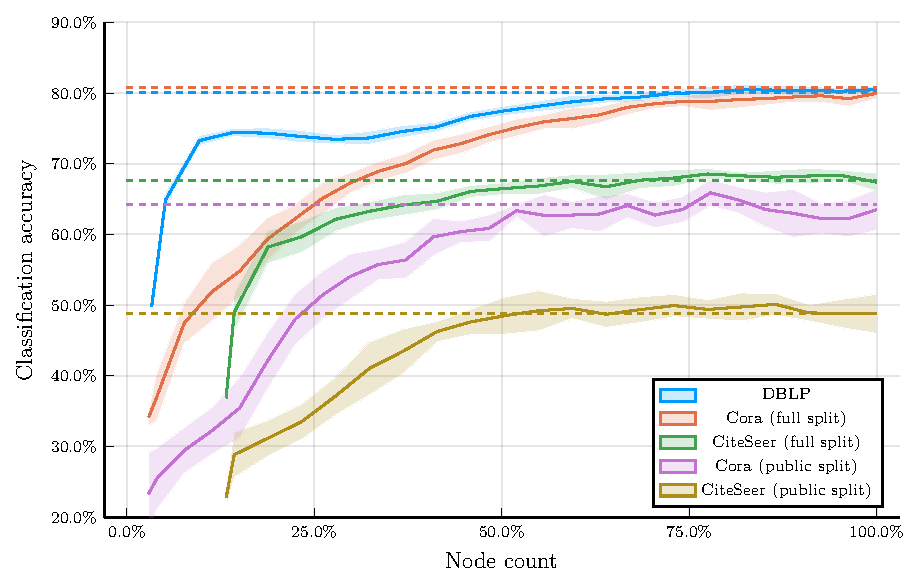
\includegraphics[width = \linewidth]{images/adaptive-coarsening/adaptive-coarsening.pdf}
  \caption{Downstream classifier accuracies at different steps of adaptive prolongation using the basic HARP coarsening algorithm. Dashed line shows the baseline node2vec model accuracy. The node count is taken relative to the total node count in each dataset. The results are averaged over multiple runs, with the solid line representing the mean and the shaded area denoting one standard deviation.}
  \label{fig:adaptive-coarsening}
\end{figure}

The behaviour of the model somewhat differs between the used datasets. For each dataset, the model starts from a very low performance, which quickly rises as the model trains for several prolongation steps. The model trained on CiteSeer attains performance comparable to the reference model when approximately half of all nodes are available to it. On the other hand, with Cora, the model slowly approaches the reference model for the whole duration of training, only reaching comparable performance at a point where nearly the whole graph is available to it. Models trained on the two larger datasets, DBLP and PubMed, exhibit a substantially different behaviour. Both models reach a local maximum at around 14\% of the graph, followed by a slight decline and gradual approach to the baseline. This suggests a global structure in the data, which the model learns at the point of the local maxima. After that point, this global structure may be obscured due to noise in the added data. The Enzymes dataset is substantially different yet again, with only small performance gains with increasing number of nodes available, however, the results contain a lot of noise, as the algorithm performace varies greatly over the different testing datasets for both the baseline as well as the adaptive prolongation approach. Of a particular note is the relatively decent accuracy even after the first prolongation step. Given the properties of the graph coarsening, this may suggest correlation between node labels of the individual graphs, which would indeed make even the coarsest step have a decent performance.

To further study the model properties, the Friedman two-way analysis of ranks was used, with the Holm-Bonferroni correction for multiple hypotheses testing. The hypotheses tested were that the resulting accuracy is the same from the \( k \)-th decile of the node count to the full graph, with tests for all possible values of \( k \). The hypotheses were tested against the 20 testing graphs from the Enzymes dataset, as well as Cora, CiteSeer, DBLP and PubMed. None of the hypotheses were rejected by the test at the 5\% level of significance. We attribute this mainly to the Enzymes dataset, which introduces a lot of noise into the data.

\subsection{Comparison of coarsening approaches}

To compare the proposed coarsening algorithms, they were trained on the Enzymes, Cora and CiteSeer datasets. This limitation is due to the GDC algorithm, which constructs a dense matrix \( S \) as part of the process, which is computationally demanding. There exists an approximate version of the algorithm, however, it is currently not implemented for the chosen combination of diffusion, normalization and sparsification methods. An extension of this approximate solution to cover all combinations of these parameters is possible, however, outside of the scope of this work.

For GDC coarsening, only the top-\( k \) sparsification method produces reliable results as thresholding leads to instability in the coarsening process, either collapsing the whole graph almost immediately, or not collapsing it at all. As for the other parameters, we followed \cite{gasteiger_diffusion_2019} and have chosen symmetric normalization for the input matrix and column normalization for the output matrix. Both of the diffusion methods propsed in \cite{gasteiger_diffusion_2019} were implemented with the recommended parameter values, that is the heat kernel was used with the diffusion time \( t = 5 \) and the Personalized PageRank algorithm with the teleport probability \( \alpha = 0.15 \).

For the evolutionary coarsening, the experimental evaluation was conducted with crossover probability \( p_\mathrm{cx} = 0.9 \), individual and gene mutation probabilities \( p_\mathrm{mut} = p_\mathrm{gene} = 0.1 \), parent population size \( \lambda = 3 \), tournament size \( n_\mathrm{tourn} = 3 \), and the individual length \( L \) set to \( 5\% \) of the input graph node count. The set \( \mathspace{AC} \) consisted of 16 atomic coarsenings (Table \ref{tab:atomic-coarsenings}). Only four of them had hyper-parameters. These were initialized by random sampling where \( d_\mathrm{lower} \) and \( d_\mathrm{upper} \) were sampled from a Poisson distribution with \( \mu = 30 \) and \( k \) and \( l \) were sampled uniformly from the set of all features. The evolutionary coarsening algorithm was implemented in the DEAP framework \cite{fortin_deap_2012}.

\begin{table}
    \caption{The atomic coarsening functions}
    \label{tab:atomic-coarsenings}
    \begin{tabularx}{\linewidth}{Xr}
        \toprule
        \textbf{Set \( \mathcal{C} \) of edges to contract}                                                                     & \textbf{Parameters}    \\
        \midrule
        A random edge                                                                                                           &                        \\
        A random edge incident to the highest degree node                                                                       &                        \\
        Edges of a random triangle                                                                                              &                        \\
        The edge whose incident nodes share the highest number of common neighbours                                             &                        \\
        The edge whose incident nodes share the lowest number of common neighbours                                              &                        \\
        A random edge whose incident nodes are adjacent to the highest degree node                                              &                        \\
        A random node of degree at least \( d_\mathrm{lower} \) and its random neighbour                                        & \( d_\mathrm{lower} \) \\
        A random node of degree at most \( d_\mathrm{upper} \) and its random neighbour                                         & \( d_\mathrm{upper} \) \\
        The edge whose incident nodes have the most neighbours in total                                                         &                        \\
        The edge whose incident nodes have the least neighbours in total                                                        &                        \\
        The edge whose incident nodes have the most similar \( k \)-th feature                                                  & \( k \)                \\
        The edge whose incident nodes have the least similar \( l \)-th feature                                                 & \( l \)                \\
        The edge whose incident nodes have the most similar features under the \( L^2 \) distance                               &                        \\
        The edge whose incident nodes have the least similar features under the \( L^2 \) distance                              &                        \\
        The edge whose incident nodes have the most similar set of features of 1-hop neighbours (under the Hausdorff distance)  &                        \\
        The edge whose incident nodes have the least similar set of features of 1-hop neighbours (under the Hausdorff distance) &                        \\
        \bottomrule
    \end{tabularx}
\end{table}

\begin{figure}
  \centering
  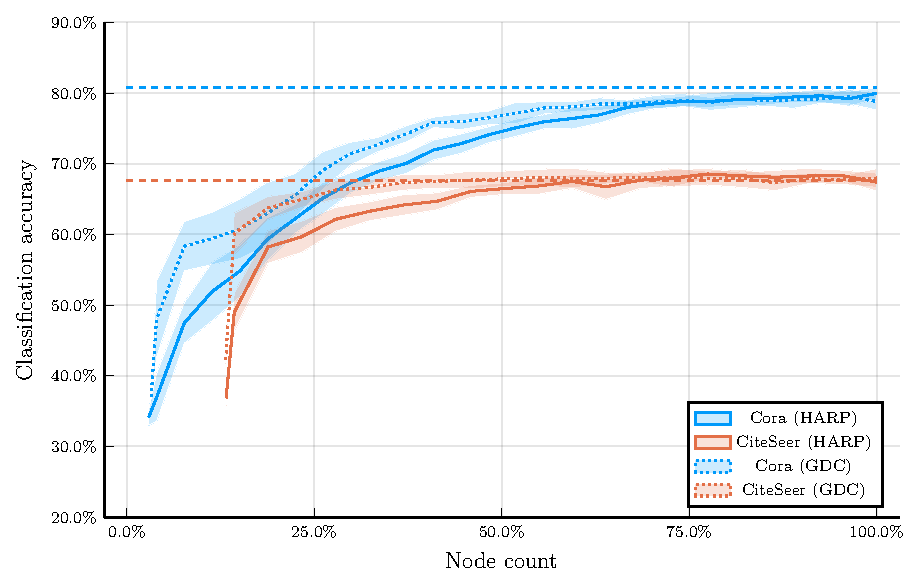
\includegraphics[width=\linewidth]{images/coarsening-algorithms/coarsening-algorithms.pdf}
  \caption{Downstream classifier accuracies at different steps of adaptive prolongation for different coarsening algorithms. Dashed line shows the baseline node2vec model accuracy. The node count is taken relative to the total node count in each dataset. The results are averaged over multiple runs, with the solid line representing the mean and the shaded area denoting one standard deviation.}
  \label{fig:coarsening-algorithms}
\end{figure}

The behaviour of the models (Figure \ref{fig:coarsening-algorithms}) again differs substantially between the datasets. As in the previous experiment, the Enzymes dataset contains a lot of noise and generally, the methods behave in a similar manner, retaining decent performance even with at the coarsest levels and only improving slightly as more data is available. At the same time, for both the Cora and the CiteSeer dataset, a clear trend emerges where the GDC coarsening quickly outperforms the original HARP coarsening, with PPR producing better results on Cora under heavy coarsening and both having similar behaviour on CiteSeer. The larger portions of the data the algorithms see, the more the margin shrinks until it vanishes completely. This suggests that the GDC algorithm is able to better preserve the global structure of the graph over successive coarsenings. On the other hand, the evolved coarsening clearly performs the worst, being outperformed by all other methods.

An identical statistical test to the one described in Section \ref{sec:adaptive-experiments} was carried out for all of the coarsening algorithms. Only the GDC coarsening with the heat kernel rejected the hypothesis that the accuracy is the same from the \( k \)-th decile onwards at the 5\% significance level, for \( k \in \left\{ 1, 2, 3 \right\} \). The Holm-corrected familywise p-values for \( k \in \left\{ 1, 2, 3, 4, 5 \right\} \) were \( 0.019, 0.023, 0.027, 0.071, 0.8 \), respectively. For other algorithms, the hypotheses weren't rejected for any value of \( k \).
